% called by main.tex
%
\chapter{Annexes}
\label{ch::Annexes}

\begin{tcolorbox}
All images presented in this report have been created manually. Images depicting infant faces have been generated using Artificial Intelligence (A1), ensuring that no real patient data or identities are compromised.
\end{tcolorbox}
\vspace{2\baselineskip}
\begin{tcolorbox}
Due to privacy and data protection laws, this project also does not include the original data identifying the babies, nor have names or any other data that could facilitate the identification of study participants or family members been released.
\end{tcolorbox}


\newpage
\section*{Research plan}

This section focuses on the temporal planning of the project. Planning a project correctly is a very important aspect as it allows for efficient time management, prioritising the most specific and relevant tasks of the project. In addition, keeping a realistic task schedule is essential to achieve the objectives set for the project within the timeframe available.

To show the time spent on each task, a Gantt Chart has been developed. This tool is widely used in project management as it allows the project schedule to be visualised, showing the tasks, their duration and the dependencies between them.

The Gantt Chart that has been made is structured by weeks and covers a total of 17 weeks, from 12/02/2024 to 07/06/2024. The weeks are detailed as follows:
\begin{itemize}
    \item Week 1: from 12/02/2024 to 18/02/2024
    \item Week 17: 03/06/2024 to 07/06/2024
\end{itemize}

This diagram includes all the main tasks that a Master's thesis project should have, as well as some specific tasks for this particular project. Thus, eight major phases have been defined, providing a clear and manageable structure for the development of the work.


\begin{figure}[h]
\centering
    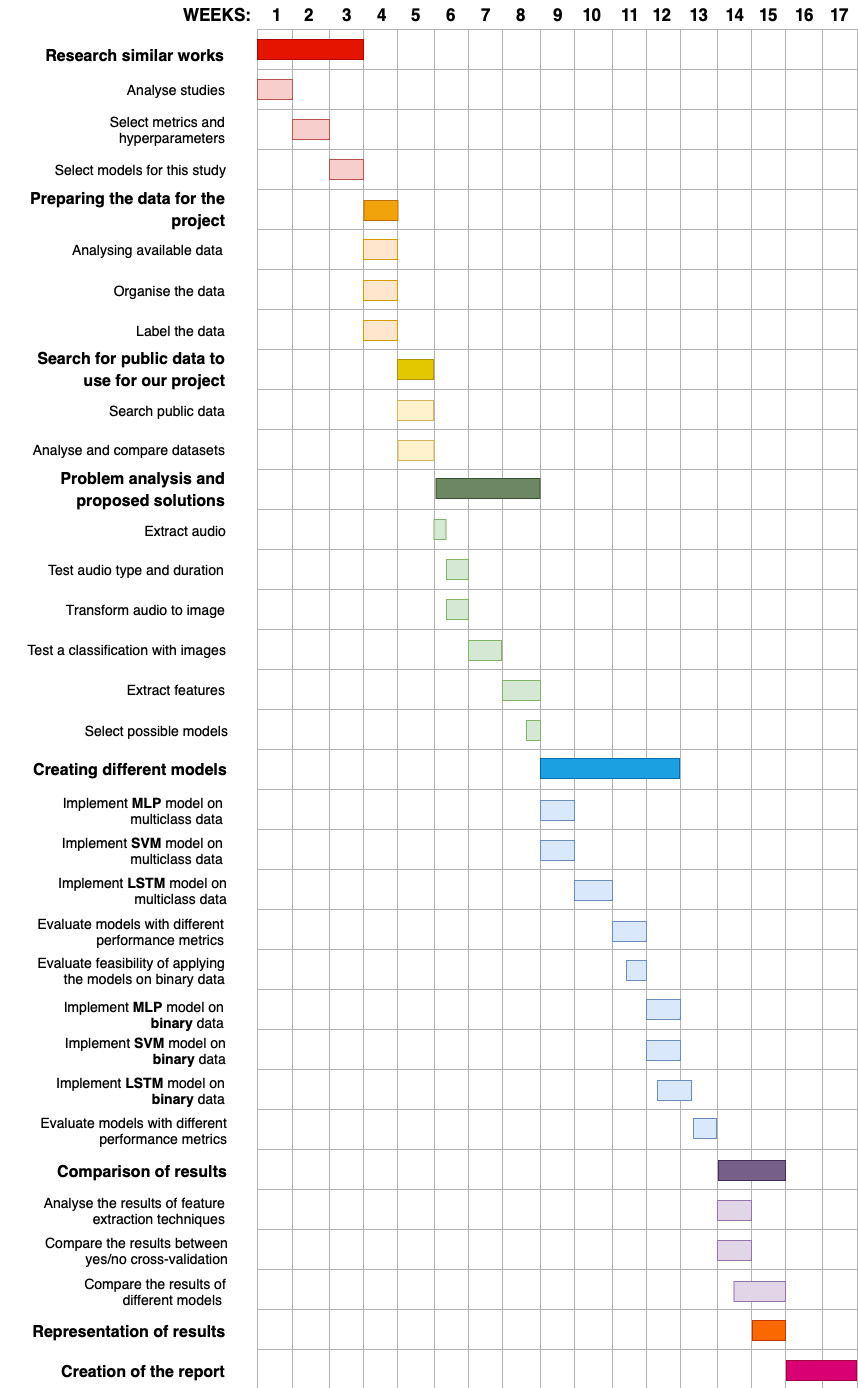
\includegraphics[width=0.8\textwidth]{figures/ChartGantt.png}
\label{fig:Gantt}
\end{figure}

